\documentclass[12pt,a4paper]{article}
\usepackage[utf8]{inputenc} % For UTF-8 encoding
\usepackage{amsmath, amssymb} % For mathematical symbols
\usepackage{graphicx} % For including images
\usepackage{hyperref} % For clickable links
\usepackage{geometry} % For page margins
\usepackage{booktabs} % For nice tables
\usepackage{lipsum} % For dummy text
\usepackage{longtable}
\usepackage{algorithm}
\usepackage{algorithmic}
\setlength{\parindent}{0em}
% Page layout
\geometry{margin=1in}

% Hyperlink setup
\hypersetup{
    colorlinks=true,
    linkcolor=blue,
    filecolor=magenta,
    urlcolor=cyan,
    pdftitle={LaTeX Template},
    pdfpagemode=FullScreen,
}

% ######################## Title  Page ####################################
\title{Recurrent Deep Learning Models and its applications}
\author{Ngai Ho Wang}

\date{\today}

\begin{document}

\maketitle
% ######################## Title  Page ####################################




% ######################## table of content ###############################
\tableofcontents % Generate a table of contents                        
% ######################## table of content ###############################

\newpage

% ######################## Project goals ######################################
\section{Project goals}
The goal of this paper is to analyze, implement, and compare the performance of RNN, LSTM, GRU and own model in selected NLP tasks. This paper aims to propose an enhanced RNN-based model for NLP tasks and make the recommendation for future development.
% ######################## Project goals ######################################


% ######################## Objectives ######################################
\section{Objectives}
\begin{enumerate}
    % 1. Literature Review
    \item Literature Review
    \begin{itemize}
        \item Conduct a comprehensive review of existing paper on RNN, LSTM, and GRU, focusing on their architecture.
        \item Review the NLP task.
    \end{itemize}

    % 2. Model implementation
    \item Model implementation
    \begin{itemize}
        \item Implement RNN, LSTM, GRU and own model by PyTorch for chosen NLP tasks.
    \end{itemize}

    % 3. Performance Comparison
    \item Performance Comparison
    \begin{itemize}
        \item Evaluate the performance by using appropriate metrics (e.g., accuracy, precision, recall, F1 score, BLEU, ROUGE).
    \end{itemize}

    % 4. Propose an advanced model
    \item Propose an advanced model
    \begin{itemize}
        \item Develop an advanced model, aiming to enhance the performance on selected NLP tasks. 
    \end{itemize}
\end{enumerate}
% ######################## Objectives ######################################

% ######################## Expected outcomes ######################################
\section{Expected outcomes}
\begin{enumerate}
    % 1. Model performance metrics
    \item Model performance metrics
    \begin{itemize}
        \item A detailed comparison of performance metrics across RNN, LSTM, GRU and own model. 
    \end{itemize}

    % 2. Practical insights
    \item Practical insights
    \begin{itemize}
        \item Practical recommendations for future work in the area of RNN applications in NLP, based on the findings of this paper. 
    \end{itemize}
\end{enumerate}
% ######################## Expected outcomes ######################################

% ######################## Research plan ######################################
\section{Research plan}
\begin{enumerate}
    % 1. Literature review
    \item Literature review
    \begin{itemize}
        \item Review existing work on RNN, LSTM, GRU and their more sophisticated variants. 
    \end{itemize}

    % 2. Model development
    \item Model development
    \begin{itemize}
        \item Select NLP tasks. (e.g., text classification, summarization).
        \item Implement baseline models (RNN, LSTM, GRU) using PyTroch.
    \end{itemize}

    % 3. Performance Evaluation
    \item Performance Evaluation
    \begin{itemize}
        \item Evaluate and compare the performance of the implemented model using appropriate metrics. 
    \end{itemize}

    % 4. Model Enhancement
    \item Model Enhancement
    \begin{itemize}
        \item Design and implement an advanced model based on findings from the previous phases.
    \end{itemize}

    % 5. Final analysis and reporting
    \item Final analysis and reporting
    \begin{itemize}
        \item Analyze the results of the advanced model against baseline models. 
    \end{itemize}
\end{enumerate}
% ######################## Research plan ######################################

% ######################## Experimental design ######################################
\section{Experimental design}
\begin{enumerate}
    % 1. Dataset selection
    \item Dataset selection
    \begin{itemize}
        \item Select suitable NLP dataset.
    \end{itemize}
    
    % 2. Model configuration
    \item Model configuration
    \begin{itemize}
        \item Define architecture specifications for each model, including number of layers, number of hidden units, activation function, dropout rates.
    \end{itemize}
\end{enumerate}
% ######################## Experimental design ######################################


\newpage
% ######################## Introduction ######################################
\section{Introduction}

With the rise of the Generative Artificial Intelligence, the development of AI has already made remarkable strides in processing sequential data. In understanding and producing sequential data. It has applications ranging from Natural Language Processing (NLP) to music composition to video generation. Especially NLP, has emerged as a pivotal field in artificial intelligence, enable machines to understand, interpret and generate in human readable format. Siri, Alexa and bixby have shown the possibility. Everyone can communicate with those machines and they with make the reasonable response to user.\\[2ex]
Recurrent Neural Networks (RNNs) have been a foundational architecture in this domain, the architecture of RNNs is design for sequential data. It able to retain the information through hidden states. Unfortunately, early RNNs had limitation in training of networks over long sequence. vanishing and exploding gradient problems significantly affect the training process of RNN (Bengio, Simard, \& Frasconi, 1994). Eliminating many practical applications of RNNs. After that, Hochreiter and Schmidhuber (1997) introduced Long Short-Term Memory (LSTM) networks and are responsible for the breakthrough in how to solve these challenges. Specificized gating mechanisms were introduced in LSTMs to regulate the flow of the information, minimize the vanishing gradient problem and learn the long-term dependencies. This advanced made RNNs much more performant on tasks like a language modeling, machine translation and speech recognition tasks.\\[2ex]
Further improvements were achieved with Gated Recurrent Units (GRUs) by Cho et al. (2014) which diminished the LSTM architecture's complexity, but still provided the same performance. GRUs performed comparably but used fewer parameters, making it computationally and more tractably trainable.
% ######################## Introduction ######################################

\newpage
% ######################## Literature Review ######################################
\section{Literature Review}
\textbf{Backpropagation Through Time}
\\[1ex]
BPTT is one of the most important algorithms used for training RNNs. Dating back to the original effort to expand the typical backpropagation algorithm, BPTT has been formulated to handle the difficulties of temporal sequences that are inherent in sequential data (Werbos, 1990). This algorithm allows RNNs in learning sequence dependent data by unfold the network over time steps and then updating weights matrix through the gradient of loss function with respect to the variable (Rumelhart, Hinton, \& Williams, 1986).
\\[2ex]
\textbf{Conceptual Framework of BPTT}
\\[1ex]
BPTT works based on the technique of treating an RNN as a deep feedforward network for across multiple time steps. In the forward pass, the RNN, like other artificial neuronal network, applies operation over the data input in sequence, bringing changes in its own state variables at every time step, depending on the input and the previous state of its general working state or hidden state. This sequential processing produces outputs and stores the internal states of the network in any period (Werbos, 1990).

This unfolds the RNN to construct a traditional Feedforward Neural Network where we can apply backpropagation through time. Below is the conceptual idea of BPTT in RNN.
\begin{figure}[h!]
    \centering
    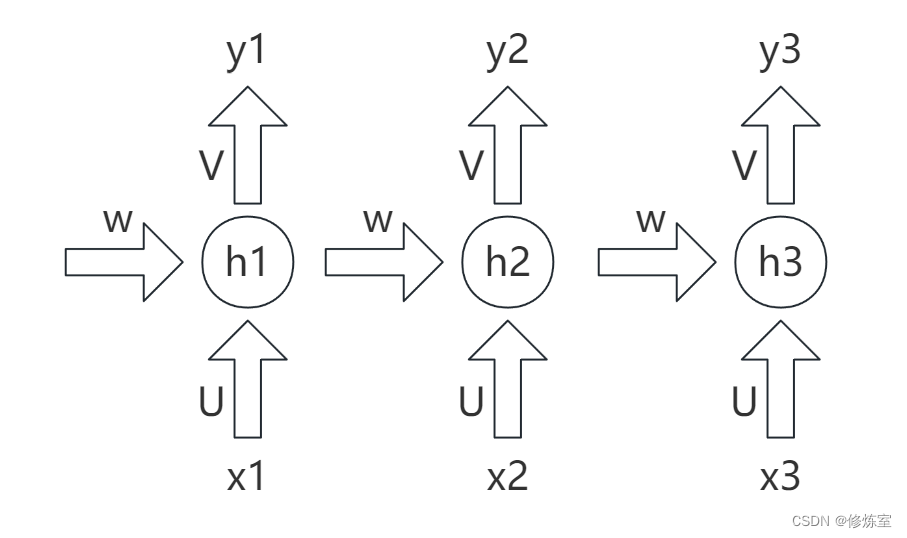
\includegraphics[width=1\textwidth]{../Pic/pic1.png} % Replace "example-image" with your image file
    \caption{Unfolded RNN}
    % \label{fig:sdfsdf}
\end{figure}

\newpage
\begin{longtable}{|c|c|c|}
    \hline
    \textbf{Notation} & \textbf{Meaning} & \textbf{Dimension}\\
    \hline
    $U$          & Weight matrix for input to hidden state       & $input\ size\times hidden\ unites$\\
    $W$          & Weight matrix for hidden to hidden state      & $hidden\ units\times hidden\ unites$\\
    $V$          & Weight matrix for hidden state to output state& $hidden\ units\times number\ of\ class$\\
    $x_t$        & Input vector at time t                        & $input\ size\times 1$\\
    $h_t$        & Hidden state output at time t                 & $hidden\ units\times 1$\\
    $b_h$        & Bias term for hidden state                    & $hidden\ units\times 1$\\
    $b_y$        & Bias term for output state                    & $number\ of\ class\times 1$\\
    $\hat{o}_y$  & Output at time t                              & $number\ of\ class\times 1$\\
    $\hat{y}_t$  & Output at time t                              & $hidden\ units\times 1$\\
    $\mathcal{L}$& Loss at time t                                & $scalar$\\
    \hline
    \caption{Unfolded RNN}
\end{longtable}

% Forward pass
\noindent \textbf{Forward Pass}
\\[1ex]
During the forward pass, the RNN processes the input sequence sequentially, computing hidden states and output at each timestep:
\begin{equation}
    h_t = f(U^Tx_{t}+W^Th_{t-1}+b_h)
\end{equation}
\begin{equation}
    \hat{y}_t = f(V^Th_t+b_y)
\end{equation}
% \begin{equation}
%     \hat{y}_t = f(\hat{o}_t)
% \end{equation}
\newline  % Computing the loss function
\noindent \textbf{Computing the loss function}
\\[1ex]
Assuming the loss is computed only at the final timestep t:
\begin{equation}
    \mathcal{L}_t = L(y_t, \hat{y}_t)
\end{equation}
In order to do backpropagation through time to tune the parameters in RNN, we need to calculate the partial derivative of loss function $\mathcal{L}$ with respect to the differently parameters.\\
\newline  % Backward pass using the chain rule
\noindent \textbf{Backward pass using the chain rule}
\\[1ex]
Using the chain rule for computing the gradient.\\
Partial derivative of loss function $\mathcal{L}$ with respect to $W$ (hidden to hidden state) at time 2. 
\begin{equation}
    \dfrac{\partial\mathcal{L}_2}{\partial{W}} = \sum_{i=1}^{2}\dfrac{\partial L_i}{\partial W}
\end{equation}
\begin{equation}
    \dfrac{\partial L_i}{\partial W} = \dfrac{\partial L_i}{\partial \hat{y}_i} \cdot \dfrac{\partial \hat{y}_i}{\partial h_i} \cdot \dfrac{\partial h_i}{\partial W}
\end{equation}
\begin{equation}
    \dfrac{\partial\mathcal{L}_2}{\partial W} = \dfrac{\partial\mathcal{L}_1}{\partial\hat{y}_1}\cdot\dfrac{\partial\hat{y}_1}{\partial\hat{h}_1}\cdot\dfrac{\partial h_1}{\partial W}+\dfrac{\mathcal{L}_2}{\partial\hat{y}_2}\cdot\dfrac{\partial\hat{y}_2}{\partial\hat{h}_2}\cdot\dfrac{\partial h_2}{\partial h_1}\cdot\dfrac{\partial h_1}{\partial W}
\end{equation}

Partial derivative of loss function $\mathcal{L}$ with respect to $U$ (input to hidden state) at time 2.\\
\begin{equation}
    \dfrac{\partial\mathcal{L}_2}{\partial{U}} = \sum_{i=1}^{2}\dfrac{\partial L_i}{\partial U}
\end{equation}
\begin{equation}
    \dfrac{\partial L_i}{\partial U} = \dfrac{\partial L_i}{\partial \hat{y}_i} \cdot \dfrac{\partial \hat{y}_i}{\partial h_i} \cdot \dfrac{\partial h_i}{\partial U}
\end{equation}
\begin{equation}
    \dfrac{\partial\mathcal{L}_2}{\partial U} = \dfrac{\partial\mathcal{L}_1}{\partial\hat{y}_1}\cdot\dfrac{\partial\hat{y}_1}{\partial\hat{h}_1}\cdot\dfrac{\partial h_1}{\partial U}+\dfrac{\mathcal{L}_2}{\partial\hat{y}_2}\cdot\dfrac{\partial\hat{y}_2}{\partial\hat{h}_2}\cdot\dfrac{\partial h_2}{\partial h_1}\cdot\dfrac{\partial h_1}{\partial U}
\end{equation}

Partial derivative of loss function $\mathcal{L}$ with respect to $V$ (hidden to output state) at time 2.\\
\begin{equation}
    \dfrac{\partial\mathcal{L}_2}{\partial{V}} = \sum_{i=1}^{2}\dfrac{\partial L_i}{\partial V}
\end{equation}
\begin{equation}
    \dfrac{\partial L_i}{\partial V} = \dfrac{\partial L_i}{\partial \hat{y}_i} \cdot \dfrac{\partial \hat{y}_i}{\partial h_i} \cdot \dfrac{\partial h_i}{\partial V}
\end{equation}
\begin{equation}
    \dfrac{\partial\mathcal{L}_2}{\partial V} = \dfrac{\partial\mathcal{L}_1}{\partial\hat{y}_1}\cdot\dfrac{\partial\hat{y}_1}{\partial\hat{h}_1}\cdot\dfrac{\partial h_1}{\partial V}+\dfrac{\mathcal{L}_2}{\partial\hat{y}_2}\cdot\dfrac{\partial\hat{y}_2}{\partial\hat{h}_2}\cdot\dfrac{\partial h_2}{\partial h_1}\cdot\dfrac{\partial h_1}{\partial V}
\end{equation}

Partial derivative of loss function $\mathcal{L}$ with respect to $b_h$ (bias term in hidden state) at time 2.\\
\begin{equation}
    \dfrac{\partial\mathcal{L}_2}{\partial{b_h}} = \sum_{i=1}^{2}\dfrac{\partial L_i}{\partial b_h}
\end{equation}
\begin{equation}
    \dfrac{\partial L_i}{\partial b_h} = \dfrac{\partial L_i}{\partial \hat{y}_i} \cdot \dfrac{\partial \hat{y}_i}{\partial h_i} \cdot \dfrac{\partial h_i}{\partial b_h}
\end{equation}
\begin{equation}
    \dfrac{\partial\mathcal{L}_2}{\partial b_h} = \dfrac{\partial\mathcal{L}_1}{\partial\hat{y}_1}\cdot\dfrac{\partial\hat{y}_1}{\partial\hat{h}_1}\cdot\dfrac{\partial h_1}{\partial b_h}+\dfrac{\mathcal{L}_2}{\partial\hat{y}_2}\cdot\dfrac{\partial\hat{y}_2}{\partial\hat{h}_2}\cdot\dfrac{\partial h_2}{\partial h_1}\cdot\dfrac{\partial h_1}{\partial b_h}
\end{equation}

Partial derivative of loss function $\mathcal{L}$ with respect to $b_y$ (bias term in output state) at time 2.
\begin{equation}
    \dfrac{\partial\mathcal{L}_2}{\partial{b_y}} = \sum_{i=1}^{2}\dfrac{\partial L_i}{\partial b_y}
\end{equation}
\begin{equation}
    \dfrac{\partial L_i}{\partial b_y} = \dfrac{\partial L_i}{\partial \hat{y}_i} \cdot \dfrac{\partial \hat{y}_i}{\partial h_i} \cdot \dfrac{\partial h_i}{\partial b_y}
\end{equation}
\begin{equation}
    \dfrac{\partial\mathcal{L}_2}{\partial b_y} = \dfrac{\partial\mathcal{L}_1}{\partial\hat{y}_1}\cdot\dfrac{\partial\hat{y}_1}{\partial\hat{h}_1}\cdot\dfrac{\partial h_1}{\partial b_y}+\dfrac{\mathcal{L}_2}{\partial\hat{y}_2}\cdot\dfrac{\partial\hat{y}_2}{\partial\hat{h}_2}\cdot\dfrac{\partial h_2}{\partial h_1}\cdot\dfrac{\partial h_1}{\partial b_y}
\end{equation}

\textbf{parameters updates}
\begin{equation}
    W \leftarrow W - \alpha\dfrac{\partial\mathcal{L}}{\partial W}
\end{equation}
\begin{equation}
    U \leftarrow U - \alpha\dfrac{\partial\mathcal{L}}{\partial U}
\end{equation}
\begin{equation}
    V \leftarrow V - \alpha\dfrac{\partial\mathcal{L}}{\partial V}
\end{equation}
\begin{equation}
    b_h \leftarrow b_h - \alpha\dfrac{\partial\mathcal{L}}{\partial b_h}
\end{equation}
\begin{equation}
    b_y \leftarrow b_y - \alpha\dfrac{\partial\mathcal{L}}{\partial b_y}
\end{equation}

\newpage
\textbf{Pseudocode of BPTT} (Wikipedia, 2023)
\begin{algorithm}[H]
    \caption{Backpropagation Through Time (BPTT)}
    \begin{algorithmic}[1]
    \STATE \textbf{Input:} 
    \STATE \hspace{1em} Sequence of input data $\{x_1, x_2, \dots, x_T\}$
    \STATE \hspace{1em} Sequence of target outputs $\{y_1, y_2, \dots, y_T\}$
    \STATE \hspace{1em} Learning rate $\eta$
    \STATE \hspace{1em} Number of time steps to unroll $N$
    \STATE \textbf{Initialize:} Model parameters $\theta$, hidden state $h_0 = 0$
    
    \STATE \textbf{Forward Pass:}
    \FOR{$t = 1$ to $T$}
        \STATE Compute hidden state: $h_t = f(h_{t-1}, x_t; \theta)$
        \STATE Compute output: $\hat{y}_t = g(h_t; \theta)$
        \STATE Compute loss for time step $t$: $L_t = \mathcal{L}(\hat{y}_t, y_t)$
    \ENDFOR
    
    \STATE \textbf{Backward Pass (BPTT):}
    \STATE Set total loss: $L = \sum_{t=1}^{T} L_t$
    \FOR{$t = T$ down to $1$}
        \STATE Compute gradient of loss with respect to output: $\frac{\partial L_t}{\partial \hat{y}_t}$
        \STATE Backpropagate through output layer to obtain: $\frac{\partial L_t}{\partial h_t}$
        \STATE Accumulate gradients for parameters: $\frac{\partial L}{\partial \theta}$
        \FOR{$k = 1$ to $N$}
            \STATE Backpropagate through time for $N$ steps:
            \STATE Compute gradient contribution from step $t-k$: $\frac{\partial L_t}{\partial h_{t-k}}$
        \ENDFOR
    \ENDFOR
    
    \STATE \textbf{Update Parameters:}
    \STATE $\theta = \theta - \eta \cdot \frac{\partial L}{\partial \theta}$
    
    \STATE \textbf{Output:} Updated parameters $\theta$
    \end{algorithmic}
\end{algorithm}

\newpage
% Actication function
\textbf{Activation function}
\\[1ex]
Activation functions, particularly the sigmoid function, are fundamental components of recurrent neural networks (RNNs). They transform input data into output data. A key property of these functions is their differentiability. Differentiability is crucial for the backpropagation through time (BPTT) algorithm, enabling the application of the chain rule during training. 
\begin{equation}
    Sigmoid(x) = \frac{ 1 }{ 1+e^{-x} }
\end{equation}
\begin{equation}
    Sigmoid'(x) = Sigmoid(x)(1-Sigmoid(x))
\end{equation}
Below is the sigmoid function and its derivative.
\begin{figure}[!htb]
    \centering
    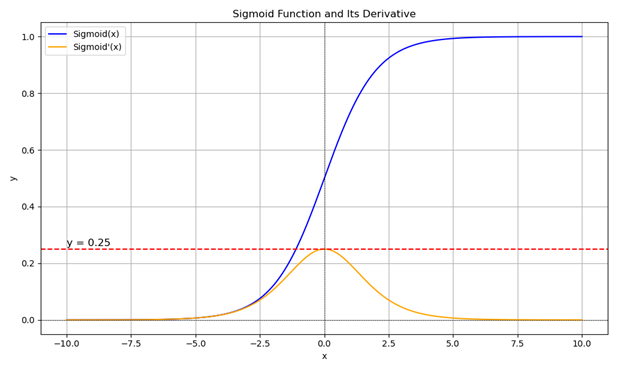
\includegraphics[width=1\textwidth]{../Pic/sigmoid.png} % Replace "example-image" with your image file
    % \caption{An example image.}
    \label{fig:sigmoid}
\end{figure}
\newline
$Domain(Sigmoid(x))=\mathbb{R},\hspace{1em} Codomain(Sigmoid(x))=(0,1)$\\
$Domain(Sigmoid'(x))=\mathbb{R},\hspace{1em} Codomain(Sigmoid'(x))=[0,0.5]$

% Hyperbolic tangent activation function
\newpage
\textbf{Hyperbolic tangent activation function}
\\[1ex]
The main role of the hyperbolic tangent (tanh) activation function is to normalize candidate values and convert the cell state to a hidden state when performing cell state updates. It limits the output between [-1,1] because it has a stable gradient, which is important for discovering long-range dependencies.
\newline
\begin{equation}
    tanh(x) = \frac{ e^{x} - e^{-x} }{e^{x} + e^{-x}}
\end{equation}
\begin{equation}
    tanh'(x) = 1 - tanh^{2}(x)
\end{equation}
Below is the Hyperbolic tangent activation function and its derivative.\\
\begin{figure}[!htb]
    \centering
    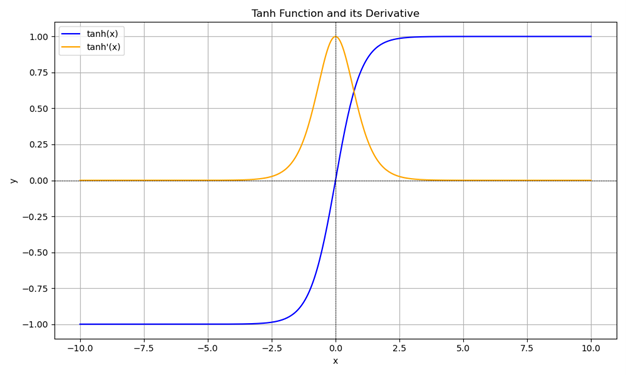
\includegraphics[width=1\textwidth]{../Pic/tanh.png} % Replace "example-image" with your image file
    % \caption{An example image.}
    \label{fig:tanh}
\end{figure}
\newline
$Domain(tanh(x))=\mathbb{R},\hspace{1em} Codomain(tanh(x))=[-1,1]$\\
$Domain(tanh'(x))=\mathbb{R},\hspace{1em} Codomain(tanh'(x))=[0,1]$

% Gradient vanishing and gradient exploring
\newpage
\textbf{Gradient vanishing and gradient exploring}
\\[1ex]
When training the RNN, BPTT was used to update the weight matrix. As the number of time steps increase, the problem of gradient instability of often encountered, and this problem is gradient vanishing and gradient explored (Bengio et al. 1994). 
\\[2ex]
% Vanishing Gradients
\textbf{Vanishing Gradients}
\\[1ex]
Generally, sigmoid activation function is used commonly in RNNs, has a maximum derivative of 0.25. When doing BPTT in long time steps, this multiplication results in exponentially diminishing gradients as the sequence length increases. Consequently, the shallow neural receive very small gradient updates, making it difficult to adjust the parameters effectively. This leads to the model struggling to learn long time dependencies. 
\\[2ex]
% Exploding Gradients
\textbf{Exploding Gradients}
\\[1ex]
When we are doing the feedforward and get super large value computed by loss function. Then when updating the parameters. The updates to the weights will also be large. Resulting in higher loss and larger gradients in the next iterations. This will lead to exploding gradients.

\newpage
% Long short-term memory (LSTM)
\textbf{Long short-term memory (LSTM)}
\\[2ex]
Long short-term memory proposed by Hochreiter \& Schmidhuber (1997). LSTM is designed for handling long time step problems. The architecture of LSTM can prevent vanishing gradient and exploring gradient. The main difference between LSTM and RNN is the number of gates. LSTM introduced input, forget and output gates. This allows LSTM to manage the flow of information more effectively, retaining important information over longer sequences.
\\[2ex]
Architecture
\\[1ex]
LSTMs introduce a memory cell that can maintain information over long time steps the cell is controlled by three gates, input gate, output gate, and forget gate. Each cell of LSTMs inside has 3 sigmoid and 1 tanh layer. Below graph unfolds the LSTM hence we can analyze different gates.
\begin{figure}[!htb]
    \centering
    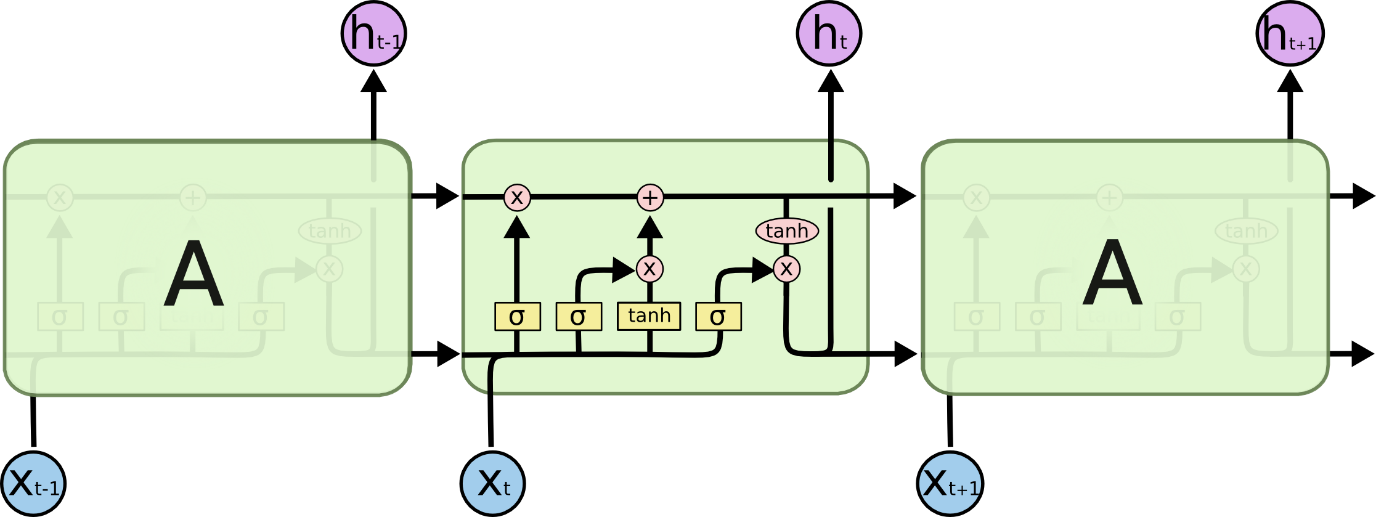
\includegraphics[width=1\textwidth]{../Pic/lstm1.png} % Replace "example-image" with your image file
\end{figure}
\begin{figure}[!htb]
    \centering
    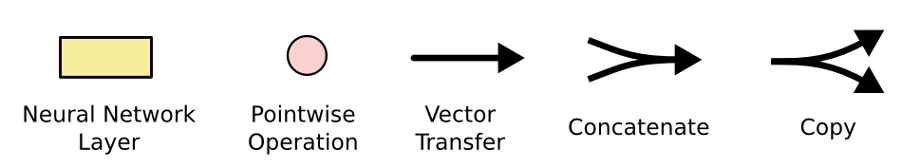
\includegraphics[width=1\textwidth]{../Pic/lstm2.png} % Replace "example-image" with your image file
\end{figure}
\\
% Forget gate
Forget gate:
\\[1ex]
The forget gate is a component of the LSTM, designed to manage the flow of information within the cell state. The function of forget gate is to determine which information should be retained in memory cell (Hochreiter, S., \& Schmidhuber, J., 1997).
\begin{equation}
    f_t = \sigma( W_f \cdot [ h_{t-1} , x_t ] + b_f ) 
\end{equation}
% Input gate
Input gate: 
\\[1ex]
The input gate controls how much new information from the current time step is allowed to enter the cell (Hochreiter, S., \& Schmidhuber, J., 1997). For the $\widetilde{C}_t$, the purpose is to suggest updates for the cell state. 
\begin{equation}
    i_t = \sigma( W_i \cdot [ h_{t-1} , x_t ] + b_c ) 
\end{equation}
\begin{equation}
    \widetilde{C}_t = tanh( W_c \cdot [ h_{t-1} , x_t ] + b_c )
\end{equation}
% Cell state update
Cell State Update:
\\[1ex]
The forget gate will drop the meaningless information and add some potential information.
\begin{equation}
    C_t = f_t * C_{t-1} + i_t * \widetilde{C_t}
\end{equation}
% Output gate
Output gate:
\\[1ex]
The output gate is able to control how much or what information from the cell state should be passed to the next layer or used in predictions. 
\begin{equation}
    o_t = \sigma( W_o \cdot [ h_{t-1} , x_t ] + b_o )
\end{equation}
% Hidden state update
Hidden State Update:
\\[1ex]
The hidden state is influenced by output value and current cell state. 
\begin{equation}
    h_t = o_t * tanh(C_t)
\end{equation}
\\[1ex]
n = number of features in the input vector $x_t$.\\
m = number of units in LSTM.\\
\begin{longtable}{|c|c|c|}
    \hline
    \textbf{Notation} & \textbf{Meaning} & \textbf{Dimension}\\
    \hline
    $x_t$               & Input vector at time t                        & $n \times 1$\\
    $h_t$               & Hidden state output at time t                 & $m \times 1$\\
    $C_t$               & Cell state at time t                          & $m \times 1$\\
    $f_t$               & Forget gate output at time t                  & $m \times 1$\\
    $i_t$               & Input gate output at time t                   & $m \times 1$\\
    $o_t$               & Output gate output at time t                  & $m \times 1$\\
    $\widetilde{C_t}$   & Candidate memory cell at time t               & $m \times 1$\\
    $W_f$               & Weight matrix for the forget gate             & $m \times (m+n)$\\
    $W_i$               & Weight matrix for the input gate              & $m \times (m+n)$\\
    $W_C$               & Weight matrix for the candidate memory cell   & $m \times (m+n)$\\
    $W_o$               & Weight matrix for the output gate             & $m \times (m+n)$\\
    $b_f$               & Bias vector for the forget gate               & $m \times 1$\\
    $b_i$               & Bias vector for the input gate                & $m \times 1$\\
    $b_C$               & Bias vector for the candidate memory cell     & $m \times 1$\\
    $b_o$               & Bias vector for the output gate               & $m \times 1$\\
    \hline
    \caption{Unfolded RNN}
\end{longtable}

Number of parameters:\\
\begin{enumerate}
    % 1. Weights matrix for the input
    \item Weights matrix for the input
    \begin{itemize}
        \item Forget gate: $n \times m$
        \item Input gate: $n \times m$
        \item Cell gate: $n \times m$
        \item Output gate: $n \times m$
    \end{itemize}

    % 2. Weight matrix for the hidden state
    \item Weight matrix for the hidden state
    \begin{itemize}
        \item Hidden state for forget gate: $m \times m$
        \item Hidden state for input gate: $m \times m$
        \item Hidden state for cell gate: $m \times m$
        \item Hidden state for output gate: $m \times m$
    \end{itemize}

    % 3. Bias term
    \item Bias term
    \begin{itemize}
        \item Bias for forget gate: $1 \times m$
        \item Bias for input gate: $1 \times m$
        \item Bias for cell gate: $1 \times m$
        \item Bias for output gate: $1 \times m$
    \end{itemize}
\end{enumerate}
Total parameters: $4 \times ( n + m + 1 ) \times m$

\newpage
% Gated Recurrent Unit (GRU)
\textbf{Gated Recurrent Unit (GRU)}
\\[1ex]
The gated recurrent unit (GRU) was proposed by Cho et al.(2014) to make each recurrent unit to adaptively capture dependencies of different time scales. The GRU has 2 gate, update gate and reset gate. 
\\[2ex]
Update gate:
\\[1ex]
The update gate determines how much of the past information should be retained in the current hidden state. 
\begin{equation}
    z_t = \sigma(W_z \cdot [ h_{t-1} , x_t ] + b_z )
\end{equation}
% Reset gate
Reset gate:
\\[1ex]
The reset gate is similar with the update gate, but the candidate hidden state is influenced by the reset gate. 
\begin{equation}
    r_t = \sigma( W_r \cdot [ h_{t-1} , x_t ] + b_r )
\end{equation}
Candidate hidden state:
\\[1ex]
The candidate hidden state combined with previous hidden state and current input to form the potential new information that can be added to the current hidden state.
\begin{equation}
    \widetilde{h_t} = tanh ( W_h \cdot [ r_t * h_{t-1} , x_t ] + b_h )
\end{equation}
Final hidden state
\\[1ex]
The final hidden state of the GRU at time t is a linear interpolation between the previous final hidden state and the candidate hidden state. 
\begin{equation}
    h_t = ( 1 - z_t ) * h_{t-1} + z_t * \widetilde{ h_t }
\end{equation}
% ######################## Literature Review ######################################




\section{Inserting Images}
asdfpiojaseopritjf
To insert an image, use the `graphicx` package. For example:

\begin{figure}[!htb]
    \centering
    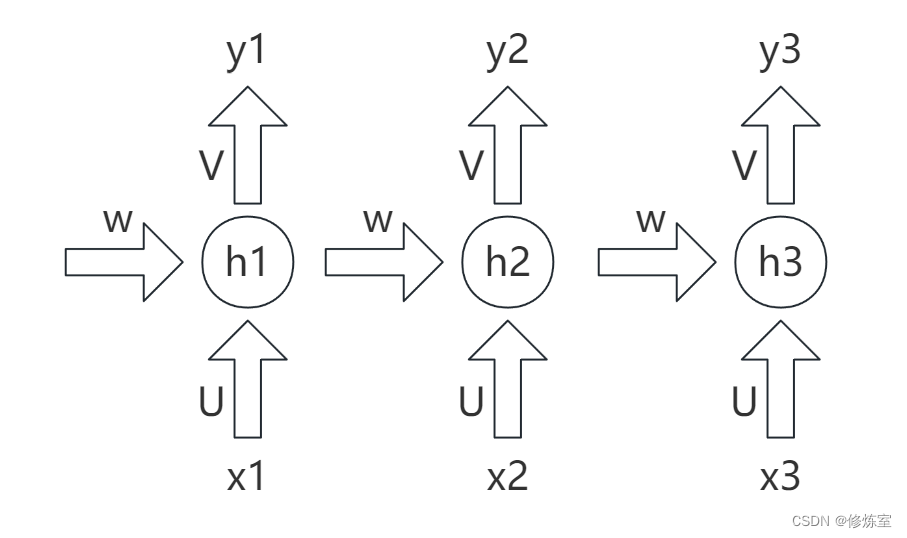
\includegraphics[width=1\textwidth]{../Pic/pic1.png} % Replace "example-image" with your image file
    \caption{An example image.}
    \label{fig:example}
\end{figure}

\section{Tables}
You can create tables using the `tabular` environment or `booktabs` for professional-quality tables. For example:

\begin{table}[h!]
\centering
\caption{Example Table}
\begin{tabular}{@{}llr@{}}
\toprule
\textbf{Item} & \textbf{Description} & \textbf{Quantity} \\ \midrule
Apples        & Fresh red apples     & 10                \\
Oranges       & Juicy oranges        & 5                 \\
Bananas       & Ripe bananas         & 7                 \\ \bottomrule
\end{tabular}
\label{tab:example}
\end{table}

\section{Hyperlinks}
To add a hyperlink, use the `hyperref` package. For example:
\href{https://www.latex-project.org/}{Visit the LaTeX project website}.

\section{Conclusions}
This is the conclusion section. Summarize your findings or leave final remarks.

\newpage
\appendix
\section{Appendix}
This is the appendix section, where you can include supplementary materials.

\end{document}